Интерфейс приложения организует работу с ассистентом. Для реализации доступного в использовании приложения был использован 
гештальт-дизайн \cite{wertheimer1938laws}, задающий правила композиции элементов интерфейса. Также были учтены
стандарты WAI-ARIA \cite{craig2009accessible}, задающие правила высокого контраста и выраженности контуров, позволяющих выполнять навигацию слабовидящим людям. 
Также функционал приложения ограничено доступен и незрячими людям, использующим специальные приложения для аудио отображения
содержания сайта.

\begin{figure}[h]
    \centering
    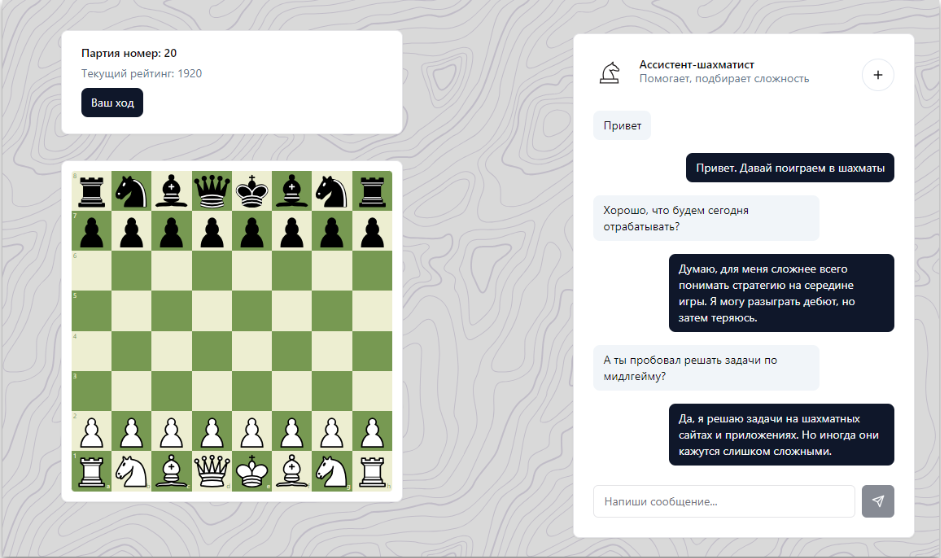
\includegraphics[width=0.5\textwidth]{assets/work/games/interface.png}
    \caption{Интерфейс имеет четкие и контрастные элементы взаимодействия. Доска для игры и диалоговое окно размещены совместно }
    \label{chess}
\end{figure}

Веб-приложение доступно при подключение через браузер по адресу доменного имени \url{www.mathema-online.xyz}. 
Технологии криптографии обеспечивают безопасность соединения, выпущенные сертификаты доменного имени 
исключают возможность подмены имени.

Интерфейс реализован с помощью популярной библиотеки React для языка программирования JavaScript \cite{ackenheimer2015introduction}.
Такой подход позволяет дескриптивно описывать элементы вебсайта, программно реагируя на взаимодействие пользователя. 
Ключевой особенностью подхода является возможность использовать открытые профессионально подготовленные интерфейсы 

При использовании данных из открытых источников используются ссылки согласно требования Гражданского кодекса
Российской федерации \cite{law1274} \cite{law1260}.



